\documentclass{article}
\usepackage{parskip}
\usepackage{pdfpages}
\usepackage[margin=.6in]{geometry}
\begin{document}
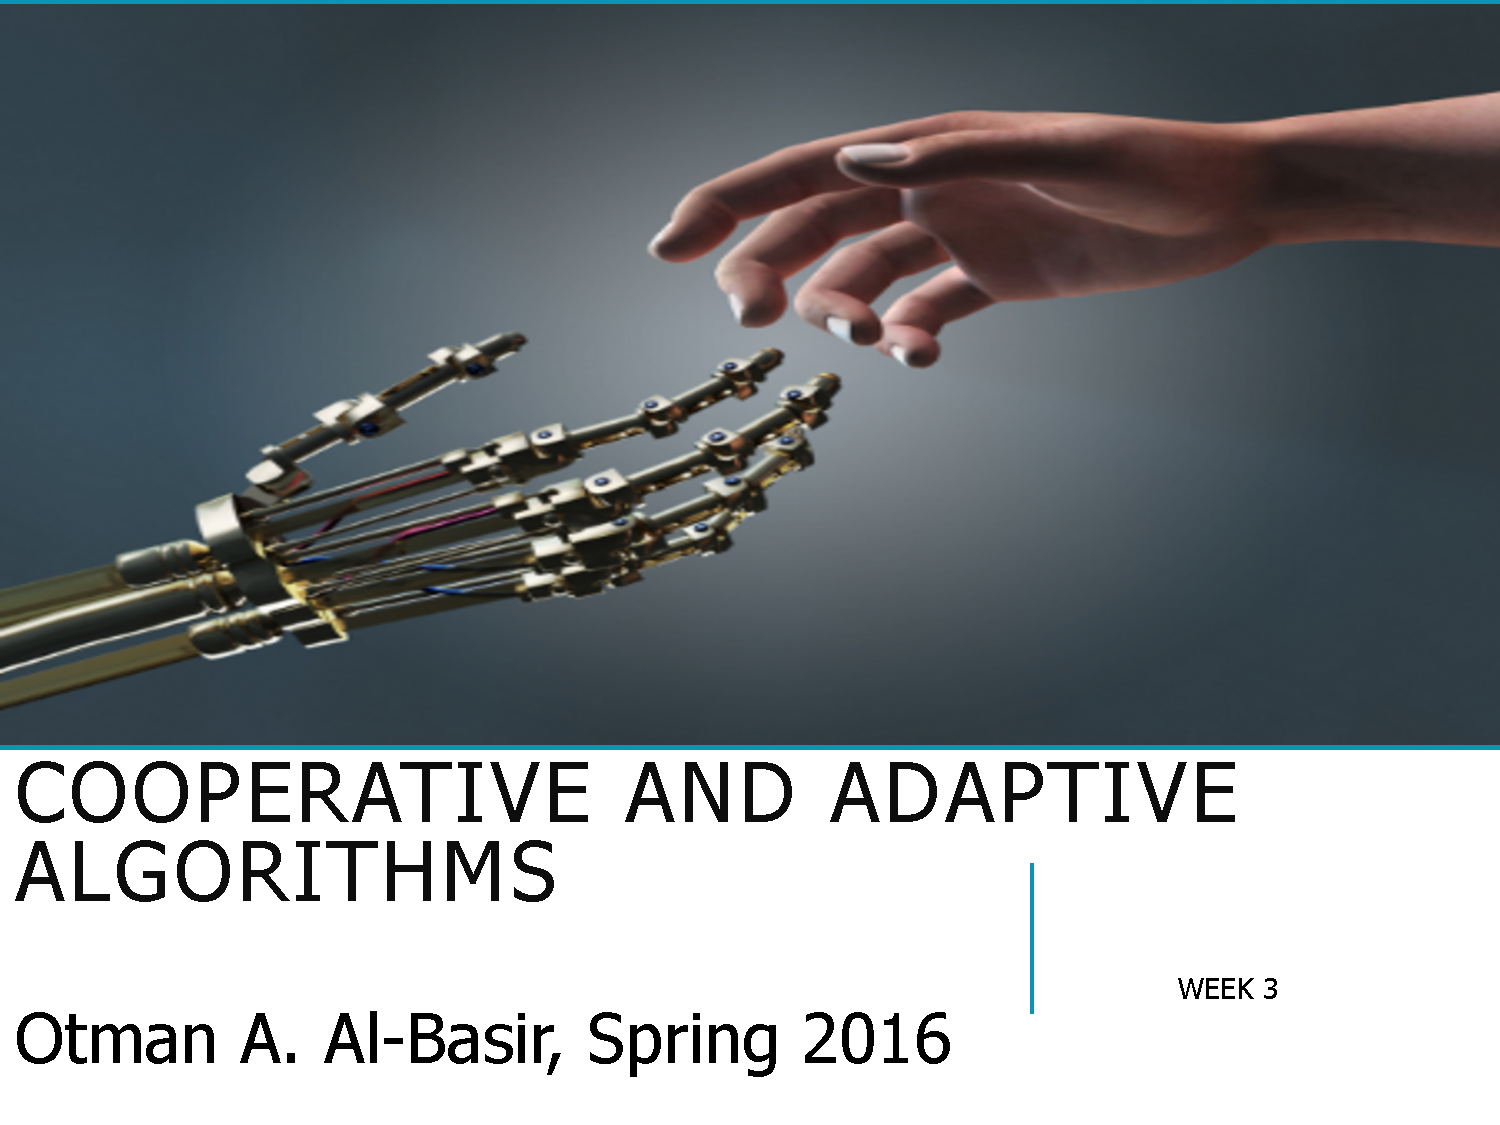
\includepdf[pages=1]{slides}
Conservation of energy, do it bitch.

\includepdf[pages=2]{slides}
For instance, if we use the known equation for kinetic energy ($\frac{1}{2}mv^2$) we can calculate the total energy before a collision and then again after. These two values are equal. Leibniz called this living force ("vis viva").

\includepdf[pages=3]{slides}
Energy can be converted to different types. For instance, when we throw a ball at a wall it is moving towards the wall, but it eventually slows to a stop. The kineic energy that it had is used to distort the shape of the ball converting the energy into elastic potential energy. This is energy stored in the electric field in the ball.

\includepdf[pages=4]{slides}
All atoms have postively and negatively charged particles in them. In the area around these particles there are electric fields

\includepdf[pages=5]{slides}
The electric field stores energy in the space between charged particles. The equation for this is $\frac{1}{2}|E|^2$. When the ball distorts in shape the kinetic energy is stored in this field (since the area is warped).

\includepdf[pages=6]{slides}
When you create a difference in charges between two plates. By putting a peice of metal between the two pieces it shorts out the fields which converts it all into kinetic energy which propels the metal really fast. It also creates plasma due to the fast amounts of energy being created.


\includepdf[pages=7]{slides}
We can use these fields to fuse particles by using the kinetic energy from a conversion from electric potential energy to squish things.

\includepdf[pages=8]{slides}
Energy can also be stored in a magnetic field $\frac{1}{2}|B|^2$. A solare flare is when the energy stored in these magnetic fields is released by the field breaking.

\includepdf[pages=9-10]{slides}
Light is electric and magnetic fields working together. Faraday found a changing magnetic field in space will created an electric field and vice versa. Maxwell is the dude that found the reverse.

\includepdf[pages=11]{slides}
Light is potential energy stored in electric and magnetic fields.

\includepdf[pages=14]{slides}
Energy can be stored in a gravitational field. For instance when you throw something up it slows down because its kinetic energy is being converted into gravitational potential energy which is stored in the gravitational field.

\includepdf[pages=15]{slides}
Solar systems are formed when a giant ball of helium and hydrogen collapses due to gravity. This results in gravitational potential converting into kinetic energy. This kinetic energy becomes thermal energy as particles collide. Eventually this becomes fusion.

\includepdf[pages=16]{slides}
Imagine a bouncy ball bouncing. You get gravitational energy to kinetic energy to elastic energy and back. But you see that the ball is not bouncing as high each time. So where is the energy going.

\includepdf[pages=17-21]{slides}
Before the ball hits the table all atoms in it have the same velocity. When it hits the table the atoms in the ball hit the atoms in the table transfering kinetic energy in random directions. Now we have disordered kinetic energy. This disordered kinetic energy comes from ordered kinetic energy (the energy we see when the ball bounces) which results in the lower bounces.

Life uses this disordered kinetic energy to do stuff. Disordered kinetic energy is called thermal energy. Life want to covert disordered kinetic energy into ordered kinetic energy.

\includepdf[pages=22]{slides}
Any item above absolute zero has its items jiggling around (thermal energy).

\includepdf[pages=23]{slides}
All objects store energy in the form of thermal energy.

\includepdf[pages=24-25]{slides}

\includepdf[pages=26]{slides}
Einstein proved that energy is equivalent to mass. The classic $E=mc^2$. He also found that space and time are unified.

\includepdf[pages=27]{slides}
Mass is the resistance of an object to changes in its motion, from here we also get the word inertia.

\includepdf[pages=28-31]{slides}
All forms of energy have mass.
If we compress a spring, adding more energy, then it becomes harder to accelerate. Its a super small number because you are diving by $c^2$. Its hard to detect, but its there. Ditto for thermal energy or electromagnetic energy. If you add light to a box full of mirrors it will be harder to accelerate.

\includepdf[pages=32]{slides}
Every particle has an anti particle that attract each other. When they collide they become pure energy. The total mass does not change even though the number of particles did. A common misconception is that the mass in the sun is converted into energy. This is not really true since the amount of mass is the same. It just converting between types of particles.

\includepdf[pages=33-39]{slides}
Mass-energy is the same thing as the warping of space time.

\includepdf[pages=40-46]{slides}
The univery is slowly approaching equilibrium at which point there will be no more flow of energy.

\includepdf[pages=47]{slides}
The logical end is the heat death of the universe which is the point at which everything is the same temperature.

\includepdf[pages=48]{slides}

\end{document}
